% !TeX root = RJwrapper.tex
\title{Techniques for Evaluating Clustering Data in R. The \pkg{Clustering} Package}
\author{by Luis Alfonso Pérez, Ángel Miguel García Vico, Pedro González and Cristóbal J. Carmona}

\maketitle

\abstract{
Clustering is an unsupervised learning technique where the model is adjusted to the observations. This technique is quite common among researchers because they can obtain knowledge quickly and easily. The use of this technique is suitable for automatically classifying data to reveal concentrations of data. This paper presents the \pkg{Clustering} package which contains a sest of clustering algorithms with two objectives: first grouping data in an homogeneous way by establishing differences between clusters, and second generating a ranking between algorithms and the variables analysed in the dataset. This package contains references to other R packages without using external software. As a complement to the standard execution through the console, it incorporates a GUI through which we can execute the package without having to know the parameters.

}

\section*{Introduction}

Exploring the properties of information in order to make groups is an unsupervised learning technique known as clustering \citep{b46} \citep{b47}. This technique is a concise data model where a set of data must be partitioned and introduced in groups or clusters of data. These clusters must meet two conditions: clusters must be the most disparate possible among them, and the elements that contain them the most similar. If we review the literature related to clustering we can see that the fields where they can be applied are multiple, among which we highlight the following: Identify tourists and analyze their destination patterns from location-based social media data \citep{b1}, \pkg{Clustering} algorithm that maximizes performance on 5G heterogeneous networks \citep{b2}, Application of data mining techniques to agriculture data \citep{b3}, Weighting of characteristics based on strength between categories and within categories for the analysis of feelings \citep{b4}, Music classification, genres and taste patterns \citep{b5}, Predict the direction, maximum, minimum and closing prices of the daily exchange rate of bitcoins \citep{b6} and \pkg{Clustering} of people in a social network based on textual similarity \citep{b7}.\\
As a rule, the clustering algorithms are based on the optimization of an objective function, which is usually the weighted sum of the distance to the centers, although these functions may vary and in some cases consists of the definition of functions. In the literature we can group the data in different ways among which we highlight \citep{b48}: partitional, hierarchical or based on density. One of the best known algorithms that solves the clustering problem is the k-means \citep{b49}\\
Throughout the literature we have located a wide variety of frameworks that work with clustering algorithm implementations among which we can cite the following: Weka \citep{b13}, ClustVis \citep{b14} and Keel \citep{b15} among others. Also within R there is a specific Cluster task view. Inside this section we see two well differentiated parts: on one hand we have the most outstanding packages by functionality and in second place we observe the set of packages that work with cluster ordered.From the set of packages we highlight the following: \pkg{ClusterR} \citep{b9}, \pkg{apcluster} \citep{b10}, \pkg{cluster} \citep{b11}, \pkg{advclust} \citep{b12} as well as alternatives to the traditional implementation of k-means and agglomerative hierarchical clustering.\\
This contribution presents the \pkg{Clustering} package. It is a package that allows you to compare multiple clustering algorithms simultaneously and assess the accuracy of the results. The purpose of this package is to evaluate a set of datasets to determine which variables have the best behavior for a series of clustering algorithms. So we can make evaluations of the clusters created, how they have been distributed, if the distributions are uniform or how they have been categorized from the data.\\
The distribution of the content of this contribution is as follows: Firstly, in section ~\ref{sec:clusteringsec} we have the  presentation of clustering, types of clustering and similarity measures is performed. Section ~\ref{sec:internalandexternalmetricssec} presents the definition of the evaluation measures in order to value the distribution of the data in the clusters and finally Section ~\ref{sec:clusteringpackage} describes the structure of the package and it presents a complete example about the use of the package.

\section*{Clustering}\label{sec:clusteringsec}

Cluster analysis is an unsupervised learning method that constitutes a cornerstone of an intelligent data analysis process. It is used for the exploration of inter-relationships among a collection of patterns, by organizing them into homogeneous clusters. It is called unsupervised learning because unlike classification (known as supervised learning), no a priori labeling of some patterns is available to use in categorizing others and inferring the cluster structure of the whole data \citep{b17}. The basic concept of clustering should be expressed as follows:
\\
\begin{quote}
\pkg{Clustering} is the process of identifying natural clusters or clusters within multidimensional data based on some measure of similarity (Euclidean, Manhattan) \citep{b18}.
\end{quote}


This is a base definition of the clustering so variations in the problem definition can be significant, depending mostly on the model specified. For example, a generative model should define similarity based on a probabilistic generative mechanism, while a distance-based approach will use a traditional distance function to quantify it. In addition, the types of data specified also have a significant impact on the problem definition.

\subsection*{Clustering types}

There are a variety of clustering algorithms that can be classified into: hierarchical (Figure \ref{fig:hierarchical}), partitioning (Figure \ref{fig:partitional}), density-based (Figure \ref{fig:density}), grid-based and probability distribution (Figure \ref{fig:model}). The most commonly used groupings are: hierarchical, part-based and density-based.
\\
\begin{itemize}
  \item Hierarchical clustering algorithms \cite{b19} create a hierarchical breakdown of data into a dendogram that recursively divides the data set into smaller and smaller data. The tree can be created in two ways: top-down or bottom-up. In bottom-up trees we can also call it agglomerative, as the objects are successively combined according to the measurements, until they are all joined into one or meet a completion condition.  In the case of top-down, it is known as divisive, where all the objects are in the same group, and as we iterate they are divided into smaller subsets, until each object is in an individual group or fulfills a condition of completion.
Some hierarchical grouping algorithms that belong to this sorting mode are CURE \cite{b20}, CHAMELEON \cite{b21}, and BIRCH \cite{b22}.
\begin{figure}[htbp]
  \centering
   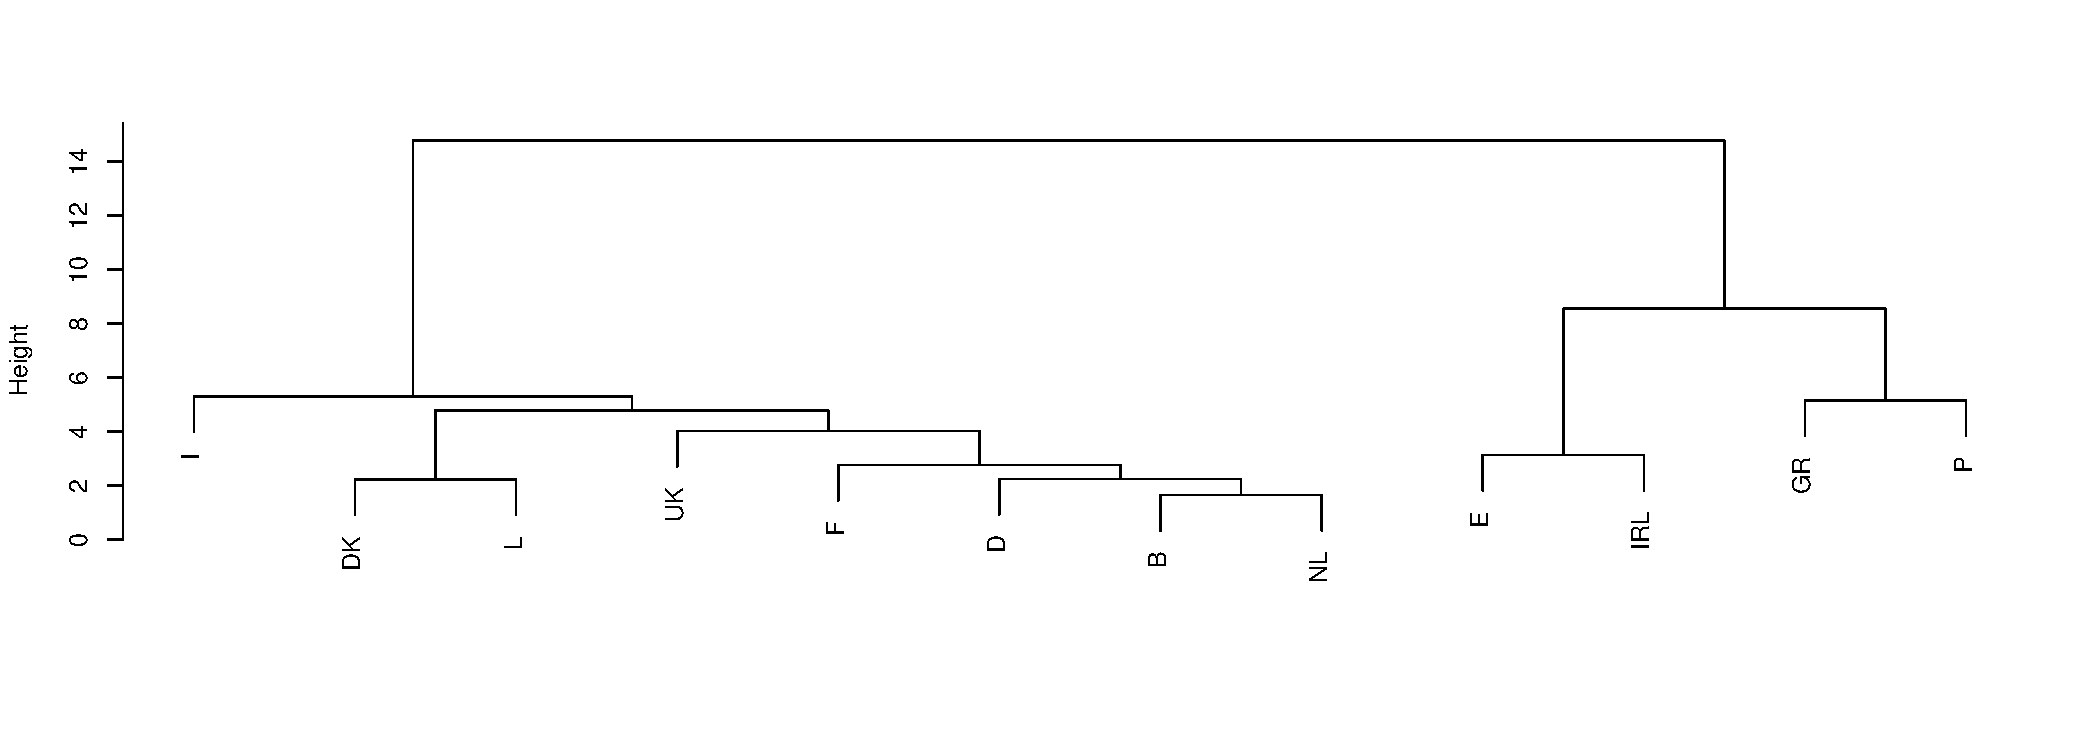
\includegraphics[width=14cm, height=5cm]{img/hierarchical}
    \caption{Hierarchical Clustering}
    \label{fig:hierarchical}%
\end{figure}
  \item Partial clustering is considered to be the most popular of the clustering algorithms \cite{b23}. Such an algorithm is also known as an iterative relocation algorithm. This algorithm minimizes a given clustering criterion by iteratively relocating data points between clusters until an optimal partition is reached. This type of algorithm divides the data points into a partition
k, where each partition represents a cluster.
Partial clustering organizes the objects within k clusters so that the total deviation of each object from the center of its cluster or from a cluster distribution is minimal. The deviation of a point can be evaluated differently according to the algorithm, and is generally known as a similarity function. Among the partitioning clustering algorithms we can find CLARANS, CLARA \cite{b24}, K-prototype \cite{b25}, K-mode \cite{b26} and K-means \cite{b27}.
\begin{figure}[htbp]
  \centering
   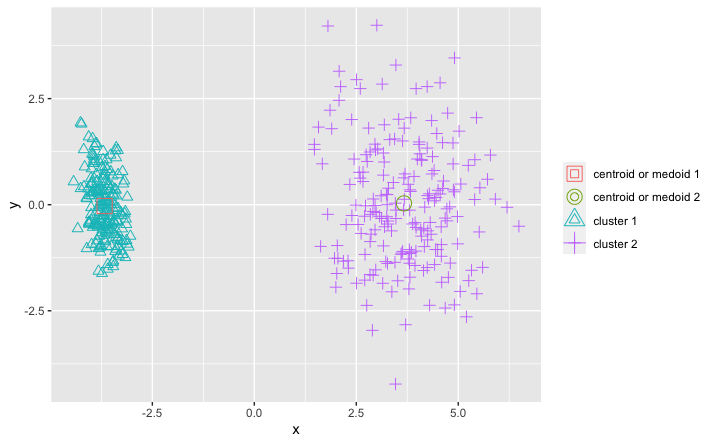
\includegraphics[width=14cm, height=5cm]{img/partitional}
    \caption{Partitional Clustering}
    \label{fig:partitional}%
\end{figure}
  \item Density-based algorithms obtain clusters based on dense regions of objects in the data space that are separated by low-density regions (these isolated elements represent noise). Among the density-based algorithms, we highlight the following: Dbscan \cite{b28}, and Denclue \cite{b29}.
  \begin{figure}[htbp]
  \centering
   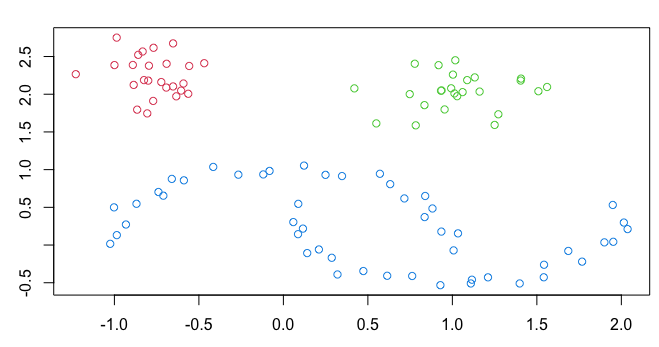
\includegraphics[width=14cm, height=5cm]{img/density}
    \caption{Density Clustering}
    \label{fig:density}%
\end{figure}
  \item Grid-based clustering algorithms \cite{b30} first quantize the clustering space into a finite number of cells and then perform the required operations on the quantized space. Cells that contain more than certain number of points are treated as dense and the dense cells are connected to form the clusters. Some of the grid-based clustering algorithms are: STING \cite{b31}, Wave Cluster \cite{b32} and CLIQUE \cite{b33}.
  \item Model-based methods are primarily based on a probability distribution. To be able to measure similarity it is based on the mean values and the algorithm tries to minimize the square error function. Auto Class algorithm uses the Bayesian approach, starting with a random initialization of parameters that is gradually adjusted in order to find the maximum probability estimates. Among the model-based algorithms SOM \cite{b34}
    \begin{figure}[htbp]
  \centering
   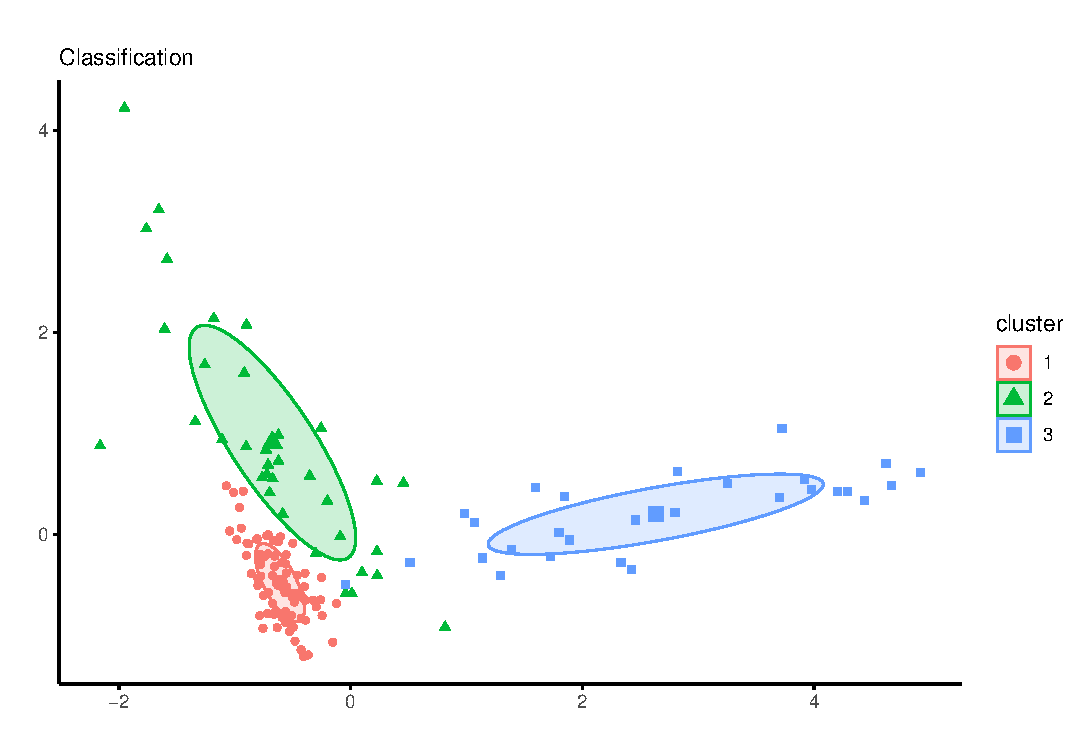
\includegraphics[width=14cm, height=5cm]{img/model}
    \caption{Model-Based Clustering}
    \label{fig:model}%
\end{figure}
\end{itemize}

\subsection*{Dissimilarity measures}

Dissimilarity measurements are important because they allow us the creation of clusters with the closest neighbours and the detection of anomalies, and they are also used in a large number of data mining techniques. It is also a measure that determines the degree to which objects are different. We often use the term distance as a synonym for dissimilarity. The values of dissimilarity should be in the range [0,1], but it is common to find in some cases the range 0 to $\infty$.
\\
Many distance measures have been proposed in literature for data clustering. The choosing an appropriate similarity measure is also crucial for cluster analysis, especially for a particular type of clustering algorithms. For example, the densit -based clustering algorithms, such as DBScan \cite{b28}, rely heavily on the similarity computation. Density-based clustering finds clusters as dense areas in the data set, and the density of a given point is in turn estimated as the closeness of the corresponding data object to its neighboring objects \cite{b50} \cite{b51}.
\\
As measures of dissimilarity in clustering we highlight the following:

\begin{itemize}
  \item Minkowski: The Minkowski family includes Euclidean distance and Manhattan distance, which are particular cases of the Minkowski distance. The Minkowski distance performs well when the dataset clusters
are isolated or compacted; if the dataset does not fulfil this condition, then the large-scale attributes would dominate the others. Another problem with Minkowski metrics is that the largest-scale feature dominates the rest.
    \begin{equation}
        d_{min} = (\sum_{i=1}^{n}|x_i - y_i|^m)^\frac{1}{m}, m\geq 1
    \end{equation}
    where m is a positive real number and xi and yi are two vectors in n-dimensional space.
    \item Euclidan distance: Is a special case of Minkowski distance. It works very well when deployed to datasets that include compact or isolated clusters. Although Euclidean distance is very common in clustering, it has a drawback: if two data vectors have no attribute values in common, they may have a smaller distance than the other pair of data vectors containing the same attribute values. Another problem with Euclidean distance as a family of the Minkowski metric is that the largest-scaled feature would dominate the others. Normalization is the solution to the problem.
    \begin{equation}
        d_{ij} =  \sqrt{\sum_{c=1}^{p}(X_{ic}-X_{jc})^2}
    \end{equation}
     \item Manhattan distance: Also known as the geometry cab driver is sensitive to outliers. When this distance measure is used in clustering algorithms, the shape of clusters is hyper-rectangular. This metric was created by Hermann Minkowski
in the 19th century and its name refers to the grid pattern of most of the streets on Manhattan Island.
     \begin{equation}
        d_{ij} =  \sum_{c=1}^{p}|X_{ic}-X_{jc}|
    \end{equation}
    \item Mahalanobis distance: Is a data-driven measure in contrast to Euclidean and Manhattan distances that are independent of the related dataset to which two data points belong. Also can be used for extracting hyperellipsoidal clusters.
    \begin{equation}
        d_{mah}= \sqrt{(x-y)S^-1(x-y)^T}
    \end{equation}
    where S is the covariance matrix of the dataset
    \item Pearson correlation: It's a statistically based metric, widely used in clustering gene expression data. This similarity
measure calculates the similarity between the shapes of two gene expression patterns.
    \begin{equation}
        Pearson(x,y)= \frac{\sum_{i=1}^n(x_i-\mu_x)(y_i-\mu_y)}{\sqrt{\sum_{i=1}^n(x_i-y_i)^2}\sqrt{\sum_{i=1}^n(x_i-y_i)^2}}
    \end{equation}
    where $\mu_x$ and $\mu_y$ are the means for x and y respectively.
    \item Jaccard Index: \cite{b35} Is a classical similarity measure on sets with a lot of practical applications in information retrieval, data mining, machine learning, and many more. Measuring the relative size of the overlap of two finite sets A and B, the Jaccard index J is formally defined as:
    \begin{equation}
        J(A,B) = \frac{A \cap B}{A \cup B}
    \end{equation}
    \item Gower distance: It is a measure of similarity that allows the simultaneous use of quantitative, qualitative and dichotomous variables. By applying this similarity coefficient can be to determine the degree of similarity between individuals; who have been measured qualitative, quantitative characteristics (continuous and discrete) and binary.
    \begin{equation}
        d_{ij}=\sqrt{(1-S_{ij})}
    \end{equation}

\end{itemize}

\section*{Internal and External clustering validation measures}\label{sec:internalandexternalmetricssec}

Clustering validation is a technique to find a set of clusters that best fits natural partitions (number of clusters) without any class information.The results of a clustering algorithm are known as cluster validity. The following criteria must therefore be taken into account when investigating the validity of clusters. The first criterion is based on external measures, which involves evaluating the results of a base algorithm in a pre-specified structure which is imposed on a data set and reflects our intuition about the structure of clustering of the data set. The second criterion is based on internal measures where it evaluates the results of a clustering algorithm in terms of the quantity involved in the vectors of the dataset itself (e.g. the proximity matrix). And as a third criterion known as relative criterion whose purpose is to compare the results of execution of an algorithm with another using different parameters.
There are two proposed criteria for the evaluation and selection of an optimal clustering \cite{b53} \cite{b52}:
\begin{enumerate}
  \item Compactness, the members of each cluster should be as close to each other as possible. A common measure of compactness is the variance, which should be minimized.
  \item Separation, the clusters themselves should be widely spaced. There are three common approaches measuring the distance between two different clusters:
  \begin{itemize}
  \item Single linkage: It measures the distance between the closest members of the clusters.
  \item Complete linkage: It measures the distance between the most distant members.
  \item Comparison of centroids: It measures the distance between the centers of the clusters.
\end{itemize}
\end{enumerate}
The two first approaches are based on statistical tests and their major drawback is their high computational cost. Moreover, the indices related to these approaches aim at measuring the degree to which a data set confirms an a-priori specified scheme. On the other hand, the third approach aims at finding the best clustering scheme that a clustering algorithm can be defined under certain assumptions and parameters.

Inside external tests exits some measures to evalute clustering results. Among which we highligh:


\begin{itemize}
    \item Entropy: \citep{b40} It evaluates the distribution of categories in a cluster.
    \begin{equation}
        Entropy =  \sum_{j=1}^{m} \frac{n_{j}}{n}E_{j}
    \end{equation}
    Where $n_{j}$ is the cluster size j, n is the number of clusters, and m is the total number of data points. To calculate the entropy of a data set, we need to calculate the class distribution of the objects in each group as follows:
    \begin{equation}
        E_{j} =  \sum_{i} p_{ij}log(p_{ij})
    \end{equation}

    \item Recall: \cite{b41} It indicates the proximity of the measurement results to the true value.
    \begin{equation}
         Recall(i,j) = \frac{n_{ij}}{n_{i}}
    \end{equation}
    $n_{ij}$ is the number of objects of class i that are in cluster j, $n_{j}$ is the number of objects in cluster j and $n_{i}$ is the number of objects in cluster i.
    \item Precision: \cite{b41} It refers to the dispersion of the set of values obtained from repeated measurements of one magnitude. The lower the dispersion, the higher the accuracy.
        \begin{equation}
            Precision(i,j) = \frac{n_{ij}}{n_{j}}
        \end{equation}
     $n_{ij}$ is the number of objects in class i that are in cluster j, $n_{j}$ is the number of objects in cluster j and $n_{i}$ is the number of objects in class i.
    \item F-measure: \cite{b42} It merges the concepts of accuracy and recall of the retrieved information. Therefore, we calculate the cluster accuracy and recall for each class as:
    \begin{equation}
        F-measure(i,j) = \frac{2 * (Precision(i,j) * Recall(i,j))}{(Precision(i,j) + Recall(i,j))}
    \end{equation}
    \item Fowlkes-Mallows Index: \cite{b43} It is a measure of comparison of hierarchical clustering, however it can also be used in flat clustering since it consists of the calculation of an index $B_{i}$ for each level i = 2 ,..., n-1 of the hierarchy. The measure $B_{i}$ is easily generalizable to a measure for clustering of different clusters.
    \begin{equation}
        Fowlkes = \frac{n_{11}}{\sqrt{(n_{11}+n_{10})(n_{11}+n_{01})}}
    \end{equation}
    It can therefore be said that Fowlkes is a measure that can be interpreted as the geometric mean of accuracy (ratio between the number of relevant documents recovered and the total number of documents recovered).


    \item Variation information: \cite{b43} Variation in information or distance of shared information is a measure of distance between two groups. This measure is closely related to mutual information. However, in contrast to mutual information, variation of information is a true metric, in the sense that it is due to the inequality of triangles.
    \begin{equation}
       VI = - \sum_{i}^{j} r_{ij}\left[\log\left(\frac{r_{ij}}{p_{i}}\right) +\left(\frac{r_{ij}}{q_{j}} \right)\right]
    \end{equation}
\end{itemize}

As with the external measures, we will now list the most relevant internal measures:
\begin{itemize}
    \item Connectivity: This measure reflects the extent to which items placed in the same group are considered their closest neighbours in the data space, i.e. the degree of connection of the clusters should be minimal \cite{b39}.
    \begin{equation}
        connectivity = \left[ 1\leq i \leq K \right]min\{ 1\leq j \leq K, i\not= j \} {min}\left\lbrace \frac{dist(C_i,C_j)}{max_1\leq k \leq K \lbrace diam(C_k) \rbrace }  \right\rbrace\
    \end{equation}
    \item Dunn: \cite{b44} It represents the relationship of the smallest distance between observations that are not in the same cluster and the largest distance within the same cluster.
    \begin{equation}
    dunn = min_{1\leq i \leq K}min \left\lbrace \frac{d(c_i,c_j)}{max_{1_\leq k \leq c(d(X_k))}} \right\rbrace
    \end{equation}
    \item Silhouette index: \cite{b45} The silhouette value is a measure of how similar an object is to its own cluster (cohesion) compared to other clusters (separation).
    \begin{equation}
        S = \frac{1}{N}\sum_{i=0}^{N}\frac{b_{i} - a_{i}}{max(a_{i},b_{i})}
    \end{equation}
    where $$a_{i}=\frac{1}{|C_{j}| - 1} \sum_{y\in C_{j},y\neq x_{i}}^{}\|y-x_{i}\|$$ and
    $$ b_{i} = \min\limits_{l \in H, l\neq j}^{} \frac{1}{|C_{l}|} \sum_{y \in C_{l}}^{} \| y - x_{i} \| $$ with
    $$ x_{i} \in C_{j}, H = \{h: 1 \leq h \leq K\}$$
\end{itemize}

The above evaluation measures can be grouped into families in order to evaluate the quality of the clusters. If we look at the Figure~\ref{fig:external} we can group Entropy, Recall, Precision, F-Measure, Fowlkes-Mallows Index and Variation information into three families \cite{b54}:

\begin{figure}[htbp]
  \centering
    \subfloat{{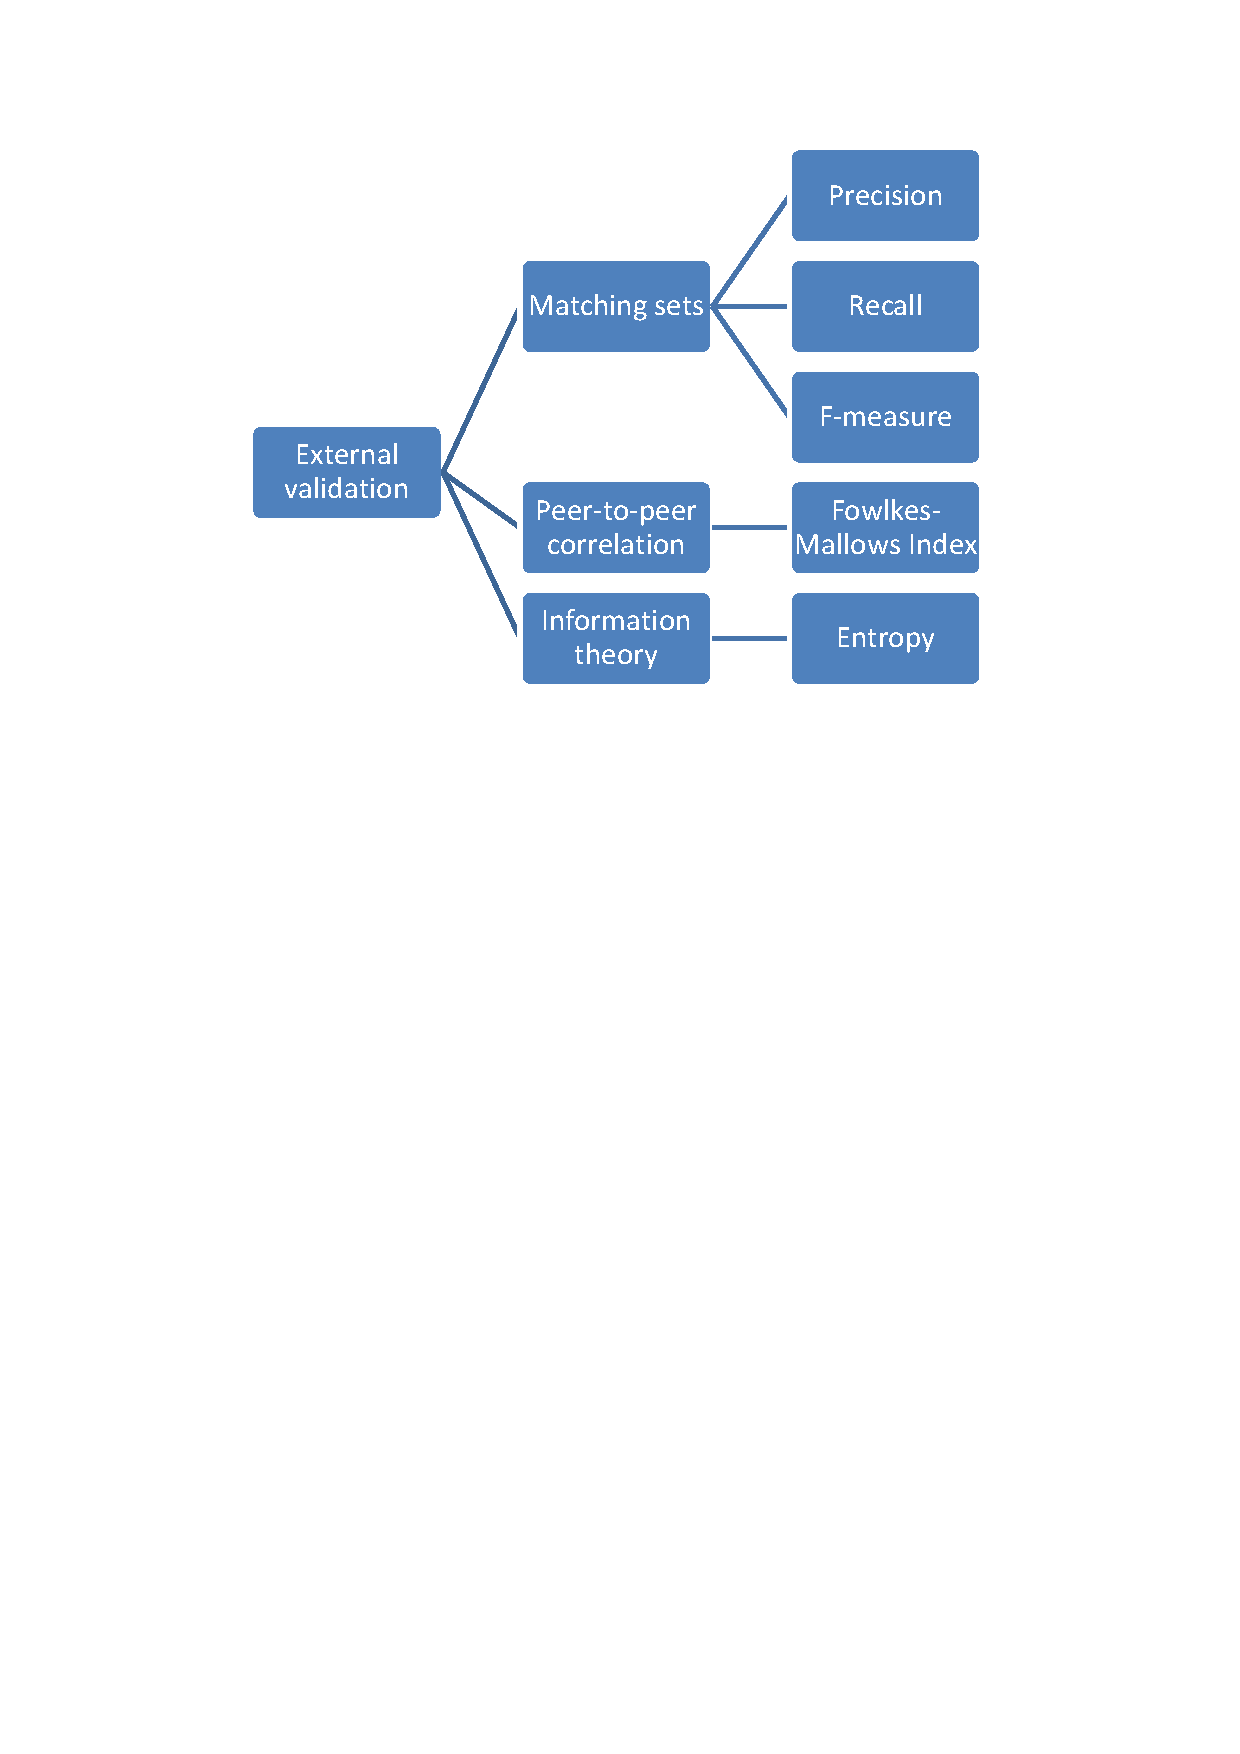
\includegraphics[width=6.5cm,height=6cm]{img/external} }}%
    \caption{External validation methods \cite{b54}}%
    \label{fig:external}%
\end{figure}

\begin{itemize}
  \item Matching Sets: \cite{b54} used to compare two partitions of data consists of those method that identify the relationship between each cluster detected in C and its natural correspondence to the classes in the reference result defined by P.\\
Several measures can be defined to measure the similarity between the clusters in C, obtained by the clustering algorithm, and the clusters if P, corresponding to our prior (external) knowledge. The metrics included in this method are: Precision, Recall and F-measure
  \item Peer-to-peer Correlation: \cite{b54} are based on the correlation between pairs, i.e. they seek to measure the similarity between two partitions under equal conditions, such as the result of a grouping process for the same set, but by means of two different methods C and P. It is assumed that the examples that are in the same cluster in C should be in the same class in P, and viceversa. We highlight the following metrics: Fowlkes-Mallows Index
  \item Measures Based on Information Theory: \cite{b54} A third family is based on Information Theory concepts, such as the existing uncertainty in the prediction of the natural classes provided by the partition P. This family includes basic measures such as entropy and variation information.
\end{itemize}

Internal evaluation metrics (see Figure ~\ref{fig:cohesion}) do not require external information, so they are focused on measuring cohesion (how close the elements are to each other) and separation (they quantify the level of separation between clusters).

\begin{figure}[htbp]
  \centering
    \subfloat{{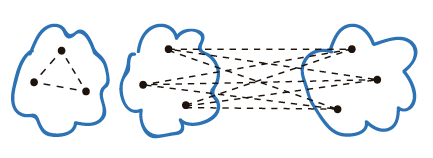
\includegraphics[width=6.5cm]{img/cohesion} }}%
    \caption{Representation of cohesion and separation in clustering \cite{b54}}%
    \label{fig:cohesion}%
\end{figure}

According to the figure ~\ref{fig:internal}, the internal Dunn, Silhouette and Connectivity metrics are based on the concepts mentioned above so we can group them as partitioning methods.

\begin{figure}[htbp]
  \centering
    \subfloat{{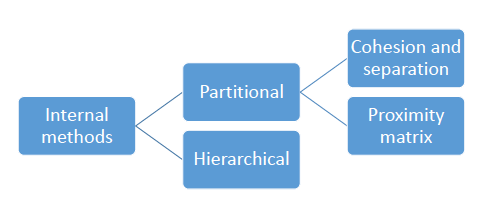
\includegraphics[width=6.5cm]{img/internal} }}%
    \caption{Internal validation methods \cite{b54}}%
    \label{fig:internal}%
\end{figure}

\section{The Clustering package}\label{sec:clusteringpackage}

\pkg{Clustering} package is a package that has been written entirely in R language. The package contains other \pkg{Clustering} packages that run hierarchical, partitional and agglomerative hierarchical algorithms. As an addition to the package it has been provided with the ability to read data in different formats such as CSV, KEEL, ARFF (Weka) and data.frame objects. Most of the methods have been provided with a set of default parameters, so we can easily run our algorithm without knowing the parameters. Later we will talk about the GUI to make the executions more attractive.

\subsection{Algorithms of the package}
These are the algorithms available within the package: \texttt{aggExCluster, agnes, apclusterK, clara, daisy, diana, fanny, fuzzy\_cm, fuzzy\_gk, fuzzy\_gg, gama, hcluster, gmm, kmeans, mona, pam, pvpick and pvclust.}

\subsection{Package Architecture}

The main advantage of this package is that it allows to compare the most used clustering algorithms in the literature and to be able to compare them to determine which variable is the best behavior for the set of algorithms. With this package we will be able to compare the results based on the best variable and evaluate the results by means of a series of metrics that will indicate how the data has been distributed within our clusters.
\\
The main class of the package is the \pkg{Clustering} object. For this we have a clustering object called \texttt{datasetTest.}
\begin{itemize}
    \item datasetTest: This object defines a dataset and contains information about it. Such information
are stored in the following fields:
    \begin{itemize}
        \item result. It represents the \texttt{data\.frame} with the results. In each column we have represented the evaluation metrics used to evaluate the clusters. We can also see the execution time of these metrics, datasets, the calculated variables, the measures of dissimilarity and the algorithms.
        \item hasInternalMetrics. It is a Boolean operator that indicates if we have used internal evaluation measures in the calculation. It serves to indicate if we have classified the data correctly.
        \item hasExternalMetrics. It is a Boolean operator that indicates if we have used external evaluation measures in the calculation.
        \item algorithms\_execute. It represents a character vector with the algorithms executed independently of the package.
        \item measures\_execute. It represents a vector of characters with the measures of dissimilarity used by the indicated algorithms.
    \end{itemize}
    This class also exports the well-known S3 methods print() and summary() that show the data
structure without codification and a summary with basic information about the dataset respectively. We can also perform sorting operations on the data in ascending and descending order. In any case if we need to perform filtering operations we can overload the operator ('[') to perform such operations in an easier way.
    \item best\_ranked\_external\_metrics: Method that looks for those external variables that are better classified, making use of the ranking column. In this way we discard the rest of the variables and only work with those that give the best response to the algorithm in question.
    \item best\_ranked\_internal\_metrics: Method that looks for those internal variables that are better classified, making use of the ranking column. In this way we discard the rest of the variables and only work with those that give the best response to the algorithm in question.
    \item evaluate\_validation\_external\_by\_metrics: The operation of this method is to determine which algorithm has better behavior regardless of the measure of dissimilarity calculated, so we can determine which algorithm returns better results from the variables and measures of dissimilarity.
    \item evaluate\_validation\_internal\_by\_metrics: The operation of this method is to determine which algorithm has better behavior regardless of the measure of dissimilarity calculated, so we can determine which algorithm returns better results from the variables and measures of dissimilarity.
    \item evaluate\_best\_validation\_external\_by\_metrics: Method that calculates the behavior of dissimilarity measures by algorithm, so we can evaluate which of the different measures of dissimilarity used by the algorithms presents the best behavior. This method should be used to determine which dissimilarity measure has the best behavior for external evaluation measures.
    \item evaluate\_best\_validation\_internal\_by\_metrics: Method that calculates the behavior of dissimilarity measures by algorithm, so we can evaluate which of the different measures of dissimilarity used by the algorithms presents the best behavior. This method should be used to determine which dissimilarity measure has the best behavior for intenal evaluation measures.
    \item result\_external\_algorithm\_by\_metric: The functionality of this method is to return as a result a data.frame with the algorithm indicated as a parameter along with the rest of the dissimilarity measurements and the external evaluation metrics.
    \item result\_internal\_algorithm\_by\_metric: The functionality of this method is to return as a result a data.frame with the algorithm indicated as a parameter along with the rest of the dissimilarity measurements and the internal evaluation metrics.
\end{itemize}
Finally we have the plot\_clustering methods to graphically represent the evaluation measurements by clusters as well as to export the results of both internal and external measurements in latex format with the export\_external\_file and export\_internal\_file methods

\subsection{Use of Clustering package}

The fastest way to download the \pkg{Clustering} package and use it is to use the install instruction.

\begin{verbatim}
install.packages("Clustering")
\end{verbatim}

A development version is also available on the github \url{https://github.com/laperez/Clustering}. To use the development version you must install the devtools package and use the install\_github method.

\begin{verbatim}
devtools::install_github('laperez/Clustering')
\end{verbatim}

The main dependencies of the \pkg{Clustering}  package are: \pkg{advclust}, \pkg{amap}, \pkg{apcluster}, \pkg{cluster}, \pkg{ClusterR}, \pkg{gmp} and \pkg{pvclust}. These are the packages in charge of implementing the clustering algorithms. We can also find dependencies for data processing and GUI, such as shiny and DT among others. Once the package is installed it is necessary to load it in the following way:

\begin{verbatim}
library("Clustering")
\end{verbatim}

Once the installation and loading process has been completed, we proceed with the processing of the data and its execution.

\subsection*{Use and load of datasets}

In the package we can see that it has a set of datasets in csv format. This dataset has been extracted from KEEL \url{https://sci2s.ugr.es/keel/category.php?cat=uns} and is in csv format. When you want to execute the algorithms of the package you can do it using the datasets defined by default, loading a dataset in memory or providing a directory where the datasets are located. On the other hand, we have a dataset called datasetTest that contains the result of the clustering algorithm execution. This dataset gives you the possibility to operate on the dataset to obtain results without the need of knowing the necessary parameters to execute the clustering method.

To see the results you can do it in the following way:
\begin{verbatim}
datasetTest
\end{verbatim}

If, on the other hand, you wish to obtain a summary of the information contained, you can do so in the following way:

\begin{verbatim}
summary(datasetTest)
\end{verbatim}

\subsection*{Execution Clustering method}

Once the way to provide the data to the clustering method has been defined, we can execute it in two ways as we have indicated above. For this example we are going to use a dataset of those provided by the package. Besides indicating the dataset, it is necessary to indicate the number of clusters, if we are going to execute all the algorithms or only those of a specific package, which measures we want to evaluate if they are internal, external or both, besides indicating if as a result we want to obtain the variables or real values. We go there with the test, we use the basketball dataset, with a range of clusters [3,5], for the gmm and target algorithm using the external metric entropy and as internal metric dunn.

\begin{Schunk}
\begin{Sinput}
> result <- clustering(df = basketball, min = 3, max = 5, algorithm = c('gmm', 'fanny'),
\end{Sinput}
\begin{Sinput}
metrics = c('entropy','dunn'))
\end{Sinput}
\begin{Soutput}
Algorithm    Distance     Clusters   Dataset   timeExternal entropy   dunn  timeInternal
     gmm   gmm_euclidean    3       dataframe    0.0054      0.2374  0.1096    0.0004
     gmm   gmm_euclidean    3       dataframe    0.0091      0.2120  0.1096    0.0005
     gmm   gmm_euclidean    3       dataframe    0.0093      0.0064  0.1096    0.0005
     gmm   gmm_euclidean    3       dataframe    0.0107      0.0032  0.1096    0.0007
     gmm   gmm_euclidean    3       dataframe    0.0185      0.0000  0.1096    0.0013
     gmm   gmm_euclidean    4       dataframe    0.0053      0.3734  0.1233    0.0004
     gmm   gmm_euclidean    4       dataframe    0.0111      0.2983  0.1233    0.0005
     gmm   gmm_euclidean    4       dataframe    0.0119      0.0064  0.1233    0.0005
     gmm   gmm_euclidean    4       dataframe    0.0122      0.0032  0.1233    0.0006
     gmm   gmm_euclidean    4       dataframe    0.0649      0.0000  0.1233    0.0007
     gmm   gmm_euclidean    5       dataframe    0.0050      0.4175  0.1619    0.0004
     gmm   gmm_euclidean    5       dataframe    0.0051      0.3857  0.1619    0.0004
     gmm   gmm_euclidean    5       dataframe    0.0086      0.0064  0.1619    0.0004
     gmm   gmm_euclidean    5       dataframe    0.0088      0.0032  0.1619    0.0005
     gmm   gmm_euclidean    5       dataframe    0.0100      0.0000  0.1619    0.0005
     gmm   gmm_manhattan    3       dataframe    0.0032      0.2498  0.1151    0.0004
     gmm   gmm_manhattan    3       dataframe    0.0038      0.2201  0.1151    0.0004
     gmm   gmm_manhattan    3       dataframe    0.0070      0.0064  0.1151    0.0005
     gmm   gmm_manhattan    3       dataframe    0.0109      0.0032  0.1151    0.0005
     gmm   gmm_manhattan    3       dataframe    0.1737      0.0000  0.1151    0.0008
     gmm   gmm_manhattan    4       dataframe    0.0031      0.3563  0.1179    0.0004
     gmm   gmm_manhattan    4       dataframe    0.0055      0.2919  0.1179    0.0004
     gmm   gmm_manhattan    4       dataframe    0.0063      0.0064  0.1179    0.0004
     gmm   gmm_manhattan    4       dataframe    0.0071      0.0032  0.1179    0.0006
     gmm   gmm_manhattan    4       dataframe    0.0096      0.0000  0.1179    0.0007
     gmm   gmm_manhattan    5       dataframe    0.0036      0.4290  0.1141    0.0004
     gmm   gmm_manhattan    5       dataframe    0.0040      0.3887  0.1141    0.0004
     gmm   gmm_manhattan    5       dataframe    0.0067      0.0064  0.1141    0.0004
     gmm   gmm_manhattan    5       dataframe    0.0076      0.0032  0.1141    0.0004
     gmm   gmm_manhattan    5       dataframe    0.0083      0.0000  0.1141    0.0005
    fanny fanny_euclidean   3       dataframe    0.0121      0.2069  0.0000    0.0000
    fanny fanny_euclidean   3       dataframe    0.0125      0.1675  0.0000    0.0000
    fanny fanny_euclidean   3       dataframe    0.0152      0.0032  0.0000    0.0000
    fanny fanny_euclidean   3       dataframe    0.0178      0.0032  0.0000    0.0000
    fanny fanny_euclidean   3       dataframe    0.0218      0.0000  0.0000    0.0000
    fanny fanny_euclidean   4       dataframe    0.0161      0.2069  0.0000    0.0000
    fanny fanny_euclidean   4       dataframe    0.0190      0.1675  0.0000    0.0000
    fanny fanny_euclidean   4       dataframe    0.0205      0.0032  0.0000    0.0000
    fanny fanny_euclidean   4       dataframe    0.0208      0.0032  0.0000    0.0000
    fanny fanny_euclidean   4       dataframe    0.0265      0.0000  0.0000    0.0000
    fanny fanny_euclidean   5       dataframe    0.0165      0.2069  0.0000    0.0000
    fanny fanny_euclidean   5       dataframe    0.0171      0.1675  0.0000    0.0000
    fanny fanny_euclidean   5       dataframe    0.0221      0.0032  0.0000    0.0000
    fanny fanny_euclidean   5       dataframe    0.0226      0.0032  0.0000    0.0000
    fanny fanny_euclidean   5       dataframe    0.0250      0.0000  0.0000    0.0000
    fanny fanny_manhattan   3       dataframe    0.0156      0.2143  0.0000    0.0000
    fanny fanny_manhattan   3       dataframe    0.0180      0.1658  0.0000    0.0000
    fanny fanny_manhattan   3       dataframe    0.0201      0.0032  0.0000    0.0000
    fanny fanny_manhattan   3       dataframe    0.0238      0.0032  0.0000    0.0000
    fanny fanny_manhattan   3       dataframe    0.0278      0.0000  0.0000    0.0000
    fanny fanny_manhattan   4       dataframe    0.0171      0.2143  0.0000    0.0000
    fanny fanny_manhattan   4       dataframe    0.0181      0.1658  0.0000    0.0000
    fanny fanny_manhattan   4       dataframe    0.0225      0.0032  0.0000    0.0000
    fanny fanny_manhattan   4       dataframe    0.0266      0.0032  0.0000    0.0000
    fanny fanny_manhattan   4       dataframe    0.0279      0.0000  0.0000    0.0000
    fanny fanny_manhattan   5       dataframe    0.0235      0.2143  0.0000    0.0000
    fanny fanny_manhattan   5       dataframe    0.0242      0.1658  0.0000    0.0000
    fanny fanny_manhattan   5       dataframe    0.0259      0.0032  0.0000    0.0000
    fanny fanny_manhattan   5       dataframe    0.0262      0.0032  0.0000    0.0000
    fanny fanny_manhattan   5       dataframe    0.0271      0.0000  0.0000    0.0000
\end{Soutput}
\end{Schunk}

If we want the best external results based on the number of clusters we can do it in the following way.
\begin{Schunk}
\begin{Sinput}
> Clustering::best_ranked_external_metrics(result)
\end{Sinput}
\begin{Soutput}
Result:
Algorithm  Distance         Clusters   Dataset  timeExternal entropy
  gmm        gmm_euclidean     3      dataframe    0.0047    0.2374
  gmm        gmm_euclidean     4      dataframe    0.0050    0.3734
  gmm        gmm_euclidean     5      dataframe    0.0059    0.4175
  gmm        gmm_manhattan     3      dataframe    0.0030    0.2498
  gmm        gmm_manhattan     4      dataframe    0.0032    0.3563
  gmm        gmm_manhattan     5      dataframe    0.0041    0.4290
fanny      fanny_euclidean     3      dataframe    0.0117    0.2069
fanny      fanny_euclidean     4      dataframe    0.0148    0.2069
fanny      fanny_euclidean     5      dataframe    0.0187    0.2069
fanny      fanny_manhattan     3      dataframe    0.0159    0.2143
fanny      fanny_manhattan     4      dataframe    0.0189    0.2143
fanny      fanny_manhattan     5      dataframe    0.0202    0.2143
\end{Soutput}
\end{Schunk}

The calculation we have done for the external evaluation measures can be done for the internal one using the following method.

\begin{Schunk}
\begin{Sinput}
> Clustering::best_ranked_internal_metrics(result)
\end{Sinput}
\begin{Soutput}
Result:
Algorithm      Distance     Clusters   Dataset  timeInternal   dunn
   gmm       gmm_euclidean     3      dataframe   0.0005      0.1096
   gmm       gmm_euclidean     4      dataframe   0.0004      0.1233
   gmm       gmm_euclidean     5      dataframe   0.0004      0.1619
   gmm       gmm_manhattan     3      dataframe   0.0004      0.1151
   gmm       gmm_manhattan     4      dataframe   0.0004      0.1179
   gmm       gmm_manhattan     5      dataframe   0.0004      0.1141
 fanny     fanny_euclidean     3      dataframe   0.0000      0.0000
 fanny     fanny_euclidean     4      dataframe   0.0000      0.0000
 fanny     fanny_euclidean     5      dataframe   0.0000      0.0000
 fanny     fanny_manhattan     3      dataframe   0.0000      0.0000
 fanny     fanny_manhattan     4      dataframe   0.0000      0.0000
 fanny     fanny_manhattan     5      dataframe   0.0000      0.0000
\end{Soutput}
\end{Schunk}

Following the analysis process we can determine which is the measure of dissimilarity that gives better results or which algorithm has better behavior for the data provided.

\begin{Schunk}
\begin{Sinput}
> Clustering::evaluate_best_validation_external_by_metrics(result)
\end{Sinput}
\begin{Soutput}
Result:
Algorithm     Distance      timeExternal entropy
 fanny     fanny_euclidean      0.0163   0.2069
 fanny     fanny_manhattan      0.0209   0.2143
  gmm       gmm_euclidean       0.0076   0.4175
  gmm       gmm_manhattan       0.0039   0.429
\end{Soutput}
\end{Schunk}
In this case we can see that the gmm algorithm with the manhattan dissimilarity measure is the one that has the best behavior when distributing the categories across all the clusters.

\begin{Schunk}
\begin{Sinput}
> Clustering::evaluate_validation_external_by_metrics(result)
\end{Sinput}
\begin{Soutput}
Result:
  Algorithm timeExternal entropy
    fanny     0.0209     0.2143
    gmm       0.0076     0.4290
\end{Soutput}
\end{Schunk}


To end the review of the external evaluation measures, we can see that the number of clusters with the best classification of the categories is k = 5

\begin{Schunk}
\begin{Sinput}
> Clustering::result_external_algorithm_by_metric(result,'gmm')
\end{Sinput}
\begin{Soutput}
Result:
Algorithm Clusters timeExternal entropy
    gmm      3       0.0045      0.2498
    gmm      4       0.0056      0.3734
    gmm      5       0.0047      0.429
\end{Soutput}
\end{Schunk}

All these operations that we have carried out to evaluate the external measures can be extrapolated to the internal ones and obtain the necessary information for the appropriate choice of the algorithm as well as the number of clusters. Another feature incorporated in the package is the possibility of being able to represent the evaluation metrics according to the number of clusters, so that in some cases you can be quite quick in choosing the best results. Figure ~\ref{fig:clustering} shows this representation

\begin{figure}[htbp]
  \centering
    \subfloat{{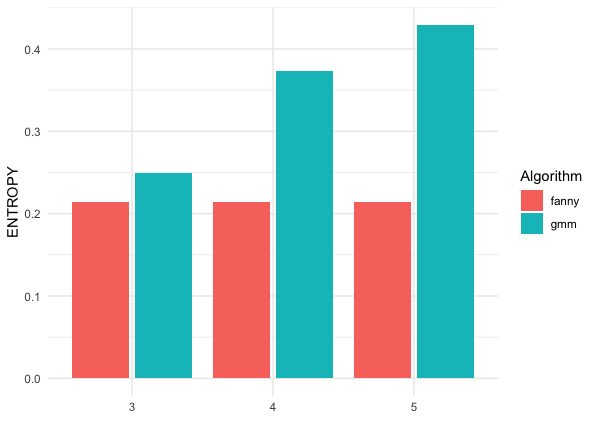
\includegraphics[width=6.5cm]{img/entropy} }}%
    \qquad
    \subfloat{{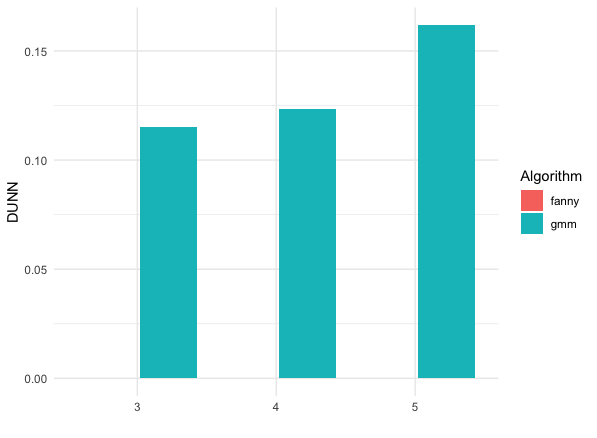
\includegraphics[width=6.5cm]{img/dunn} }}%
    \caption{Graphical representation of evaluation measures}%
    \label{fig:clustering}%
\end{figure}

\section{GUI - Grafical User Interface}

As mentioned throughout this paper, the Clustering package provides the GUI to work with clustering algorithms and to be able to evaluate and run the results more efficiently. The way to run the user interface is to execute the following instruction:

\begin{Schunk}
\begin{Sinput}
> appClustering()
\end{Sinput}
\end{Schunk}

The execution will open our default browser with the interface. As you can see in the Figure ~\ref{fig:layoutApp}, we have a layout with header, side menu and main. In the header menu we can choose to see the numerical results or in graphic mode. In the left menu we can see the different parameters with which we can run our algorithm and finally in the central menu you can see the result of running the clustering algorithm.

\begin{figure}[htbp]
  \centering
   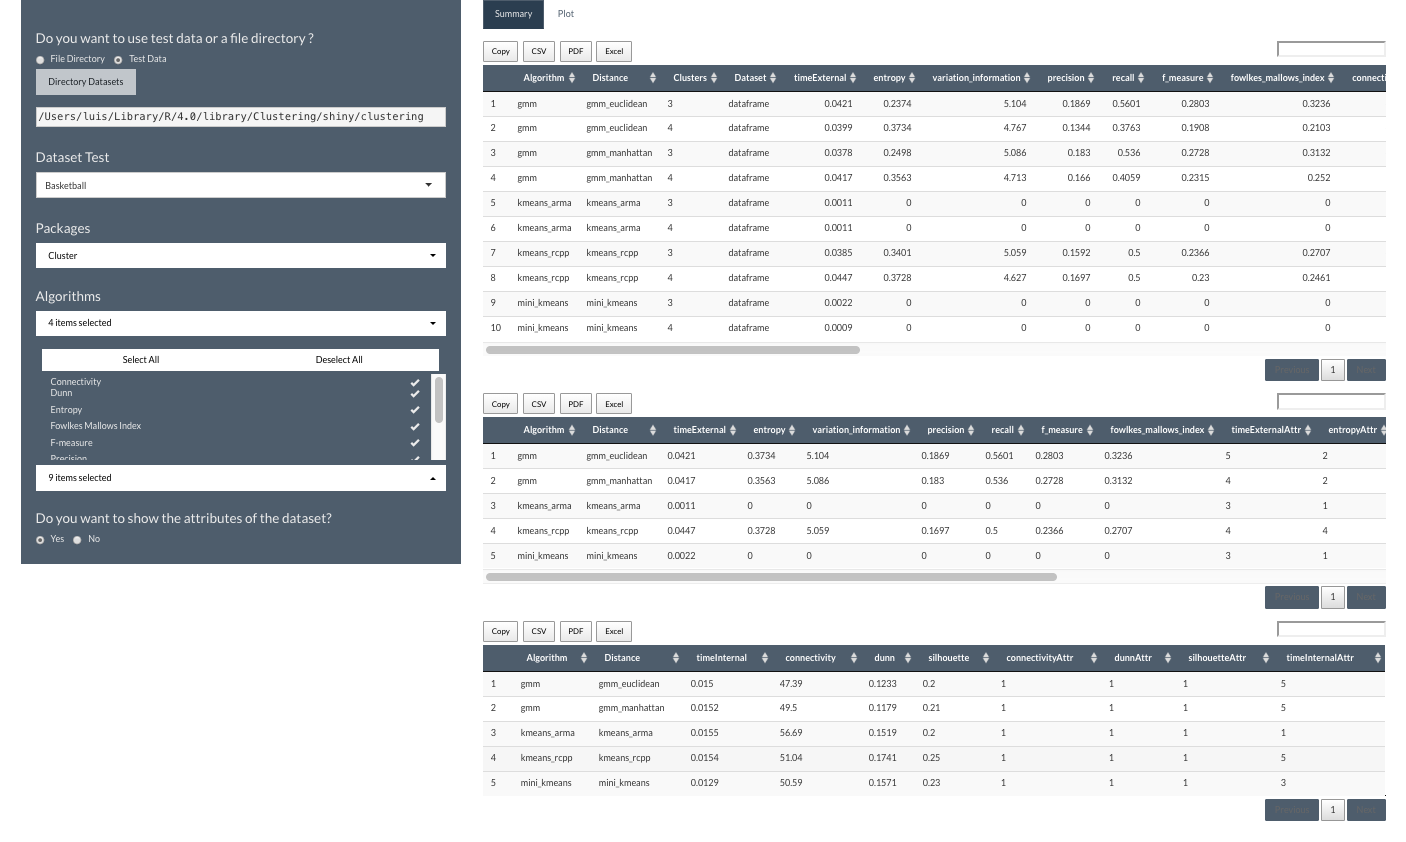
\includegraphics[width=14cm]{img/app}
    \caption{Clustering App}
    \label{fig:layoutApp}%
\end{figure}

The operation is very simple, we can choose to work with test data or file directory, work a range of clusters, specify algorithms individually or select the algorithms contained in a package, indicate what type of measures we want to evaluate and finally we can indicate if we want to see the results calculated or translate it to the variables of the dataset.
We will see this operation step by step.

\begin{figure}[htbp]
  \centering
   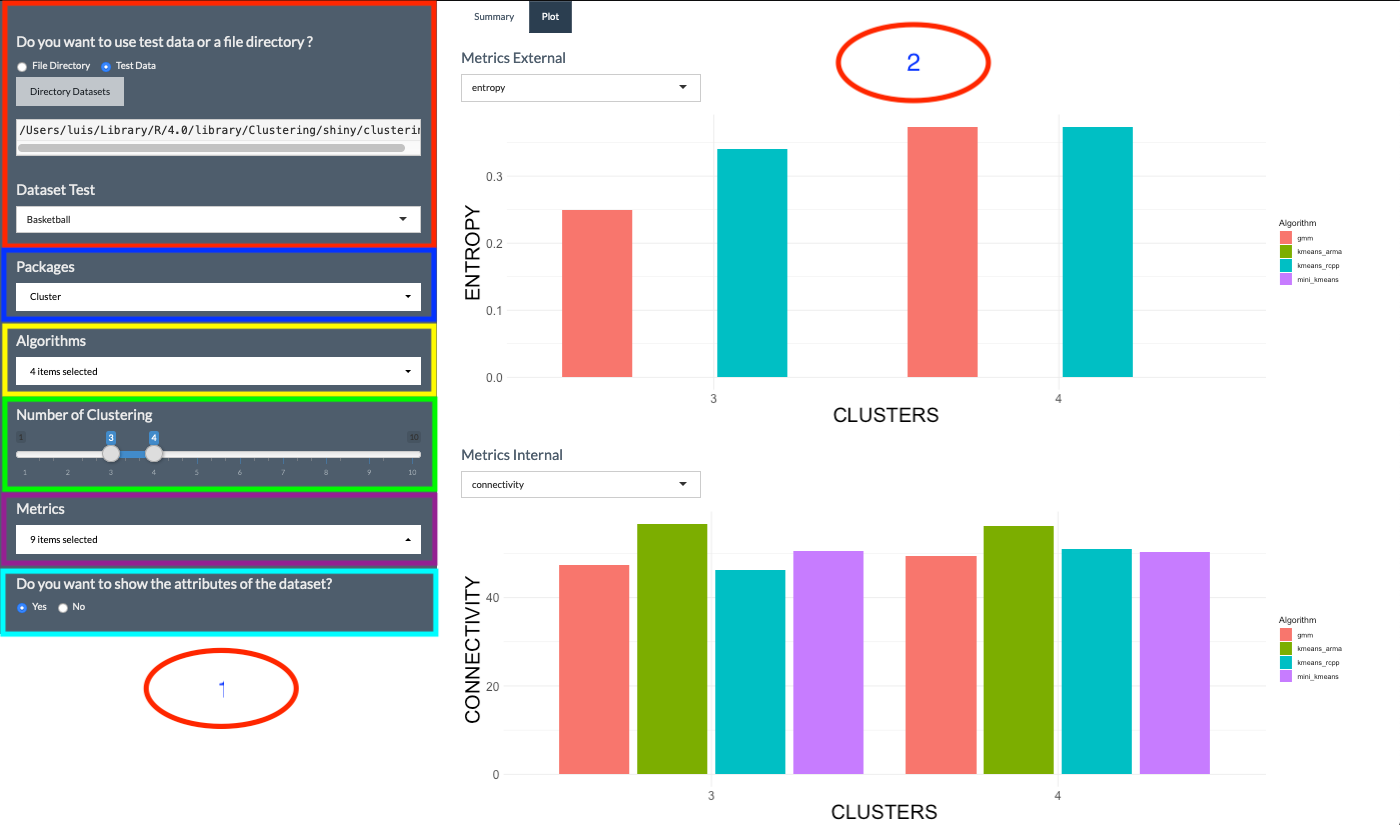
\includegraphics[width=14cm]{img/app1}
    \caption{Clustering App}
    \label{fig:layoutApp1}%
\end{figure}

As you can see in the Figure we have two well differentiated parts.
\begin{enumerate}
  \item In this section we can find the different parameters used by the clustering algorithm to filter the information.
  \begin{itemize}
  \item Marked in red, we can indicate if we want to work with test datasets or indicate a directory of dataset files to be processed.
  \item In blue we have the packages that implement the clustering algorithms mentioned throughout the paper. We can mark all the packages or individually. At the time of marking a package automatically in the combo algorithm will mark the algorithms implemented by the marked package.
  \item In yellow we have the algorithms implemented by the packages. If we mark an algorithm it will automatically mark its corresponding package in the package combo.
  \item In green we have the number of clusters. We can indicate ranges or select only one cluster by positioning the max and minimum on the same value.
  \item In violet we indicate the evaluation metrics used when validating the clusters.
  \item Finally we have a check to indicate if we want to see the results translated into the dataset variables or not.
\end{itemize}
  \item In main layout we have the options to represent the data.
  \begin{itemize}
  \item To view the data in graphical mode as shown in the Figure, we mark the Plot tab. In the figure we can see represented the internal and external evaluation metrics and depending on the type of evaluation we can filter individually by metrics to see the data represented graphically.
  \item If we click on the summary tab we can see the data represented in tables. If you wish you can export the results in the following formats: csv,pdf and xls. If you wish you can copy the results.
\end{itemize}


\end{enumerate}

\section{Summary}

In this paper we have made an introduction to the \pkg{Clustering} package. The package has dependencies with other packages as seen throughout the paper. It allows the reading and loading of datasets in KEEL, CSV or ARFF format. We also offer the functionality of loading a data.frame in memory or using test datasets. As a complement the package has been enhanced with the inclusion of a graphical interface that allows the user to run the package in a simple way without the need to know the parameters. The development of the package will be continued with the inclusion of new algorithms, functionalities and improvement of the interface, therefore we encourage developments to contribute to the improvement of the package with the inclusion of new algorithms or functionalities or the inclusion of new proposals that complement the package.

\bibliography{RJreferences}

\address{Luis Alfonso Pérez Martos\\
  Computer Department\\
  University of Jaén\\
  Spain\\
  (ORCiD if desired)\\
  \email{lapm0001@gmail.com}}

\address{Ángel Miguel García Vico\\
  Computer Department\\
  University of Jaén\\
  Spain\\
  (ORCiD if desired)\\
  \email{agvico@ujaen.es}}

\address{Pedro González\\
  Computer Department\\
  University of Jaén\\
  Spain\\
  (ORCiD if desired)\\
  \email{pglez@ujaen.es}}

\address{Cristóbal J. Carmona\\
  Computer Department\\
  University of Jaén\\
  Spain\\
  (ORCiD if desired)\\
  \email{ccarmona@ujaen.es}}
